\begin{document}
Da es sich in diesem Projekt hauptsächlich um die Visualisierung von Daten handelt, wird ein Teil diese Dokuments den Aspekten und dem
wissenschaftlichen und historischen Teil der Visualisierung von Daten gewidmet. Daten Visualisierung in der Technik ist das verwenden von
grafischen Elementen um Zusammenhänge und Muster von Datensätze zu offenbaren.  

\section{Der drang Daten zu Visualisieren}
Menschen hatten und haben seit Jahrhunderten den drang Informationen visuell Darzustellen und Festzuhalten. Die Vorgeschichte der Visualisierung
ist durch verschiedene Technologien und Bedürfnisse geprägt worden, diese variieren von Bildhauereien, Karten, Bildern bis hin zu Tabellen
von Zahlen.\\ \\
Doch die Frage lautet, warum Visualisieren wir eigentlich Daten? \\ \\
Wie schon Kurz erwähnt ist der Sinn der Daten Visualisierung, zusammenhänge zwischen Informationen, Konzepten oder Logiken dem Menschen über
eine Grafik zu zeigen und festzuhalten.  \\
Diese können von mathematischen Prozessen, Zusammenhängen bis hin zu den zusammenhängen von Ereignissen, Daten variieren. Es ist schwer
Menschen zusammenhänge Anhand von Zahlen zu verdeutlichen ganz besonders wenn es mehr dimensionale Daten sind. Doch kann man diese
Informationen aus einem gut durchdachten Grafen meist schneller, besser und einfacher extrahieren als aus Formeln oder Tabellen. \\ 
Dies hat mit unserem komplexen visuellem Kortex zu tun welches sehr gut darin ist Unterschiede in Form, Farbe und Größe zu ermitteln, wodurch
es wiederum zusammenhänge bei visuelle Informationen sehr gut erfassen und verarbeiten kann. Der bedarf Daten zu visualisieren stieg ganz
besonders mit dem Anstieg der Daten die man Heutzutage im Internet finden kann. \newpage

\section{Arten und Techniken der Visualisierung}
Über die Jahrhunderte haben sich verschiedene Techniken und Arten der Datenvisualisierung durchgesetzt. In diesem Abschnitt werde ich etwas
genauer auf Techniken und Arten von Visualisierungen eingehen. \\
Im folgenden Abschnitt werde ich eine Reihe von arten auflisten:
\begin{itemize}
    \item{Tabellen:} \\ \\
        Als eines der ältesten Formen der Visualisierung, welche wir im 21 Jahrhundert immer noch verwenden, ist die Tabelle eine gute Form der
        Visualisierung wenn man ein Gefühl für die Zahlen bekommen will. Jedoch ist es schwer einen zusammenhang zwischen Zahlen zu
        ermitteln da diese alleine stehend für sich nicht viel Aussagen.
    \item{Charts: Balken oder Kreis: } \\ \\
        Diese Form von Diagrammen geben üblicherweise zwei dimensional Daten wieder, doch kann man in der Theorie n Dimensionale Grafiken erstellen. Zum
        Beispiel Entwurf Charles Joseph Minard, ein französischer Bauingeneur, einen Grafen im Jahre 1869 welches den Marsch von Napoleon
        nach Russland in sechs Dimensionen beschrieb.\cite{bestvisualizations}
        \begin{center}
            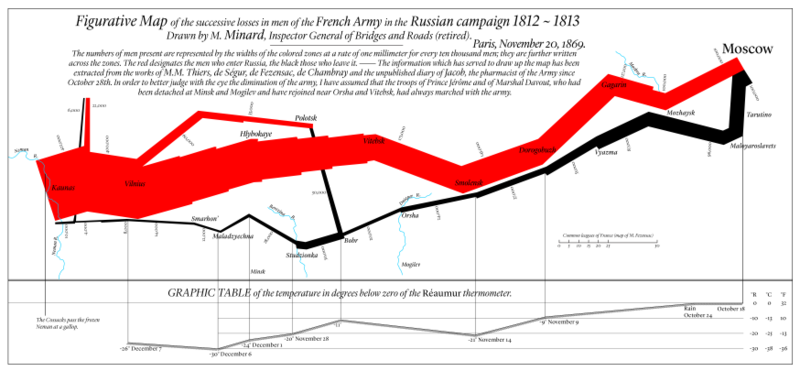
\includegraphics[width=1\textwidth]{800px-Minard_Update.png}\cite{minardgraph}
        \end{center}
        In diesem einen Grafen erfasst Minard folgende Informationen:
        \begin{itemize}
            \item Größe der Arme anhand der breite des Balken zu verschiedenen Zeiten
            \item Temperatur anhand des simplen Grafen unten
            \item Richtung des Marsches (Rot Hinweg, Schwarz: Rückweg) 
            \item Ort anhand der Karte
            \item Distanz anhand der Karte
            \item Latitude, Longitude anhand der Karte
        \end{itemize}
    \item{Ein bis drei dimensionale Diagramme:} \\ \\
        Diese Sorte von Grafen sind sehr gut wenn man die Informationen in maximal drei Dimensionen, minimal einer Dimension hat oder die
        jeweilige andere durch Anwendung von Formeln oder anderen Gegebenheiten umwandeln kann. \\
        Zum Beispiel kann man die Farbverteilung eines Bildes sehr einfach und präzise in so einem zwei oder drei dimensionalen Diagramm
        visualisieren. Für das folgende Bild wird ein 2D Histogramm generiert welches die Menge der drei Grundfarben (rot, grün, blau)
        visualisiert.
        \begin{center}
            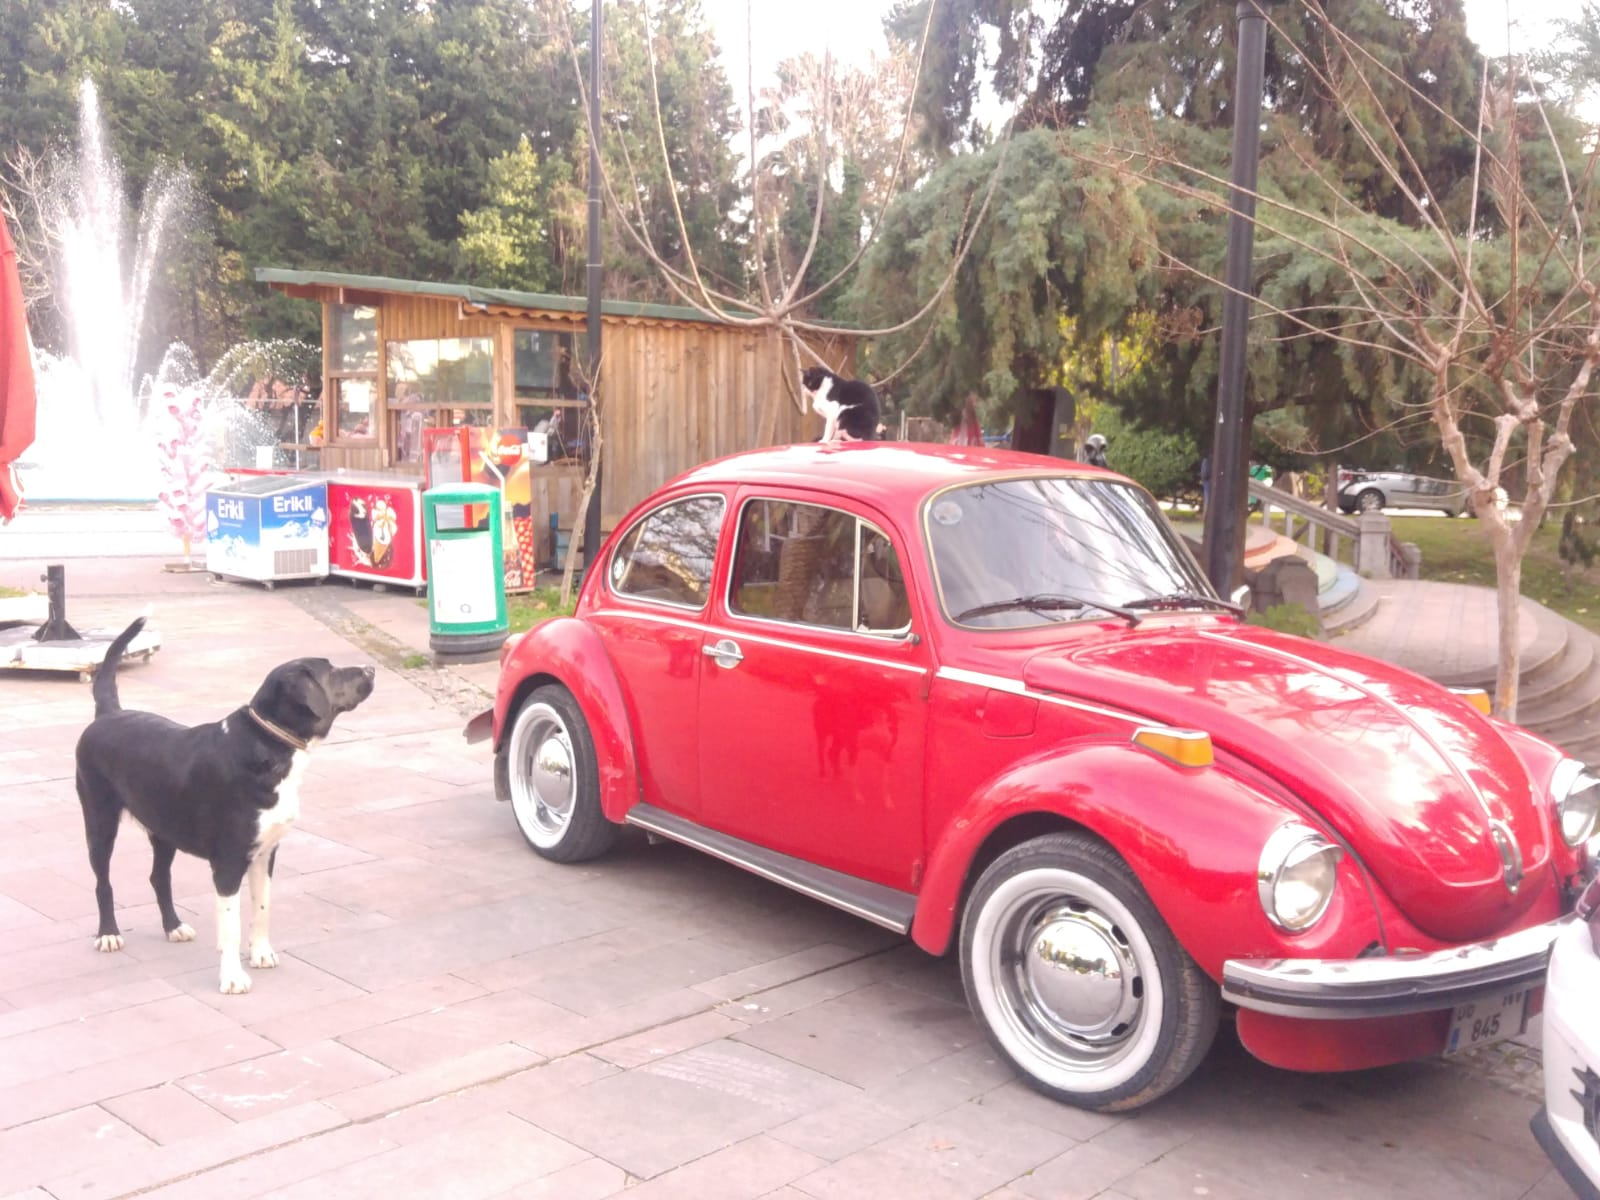
\includegraphics[width=0.75\textwidth]{image.jpg}
            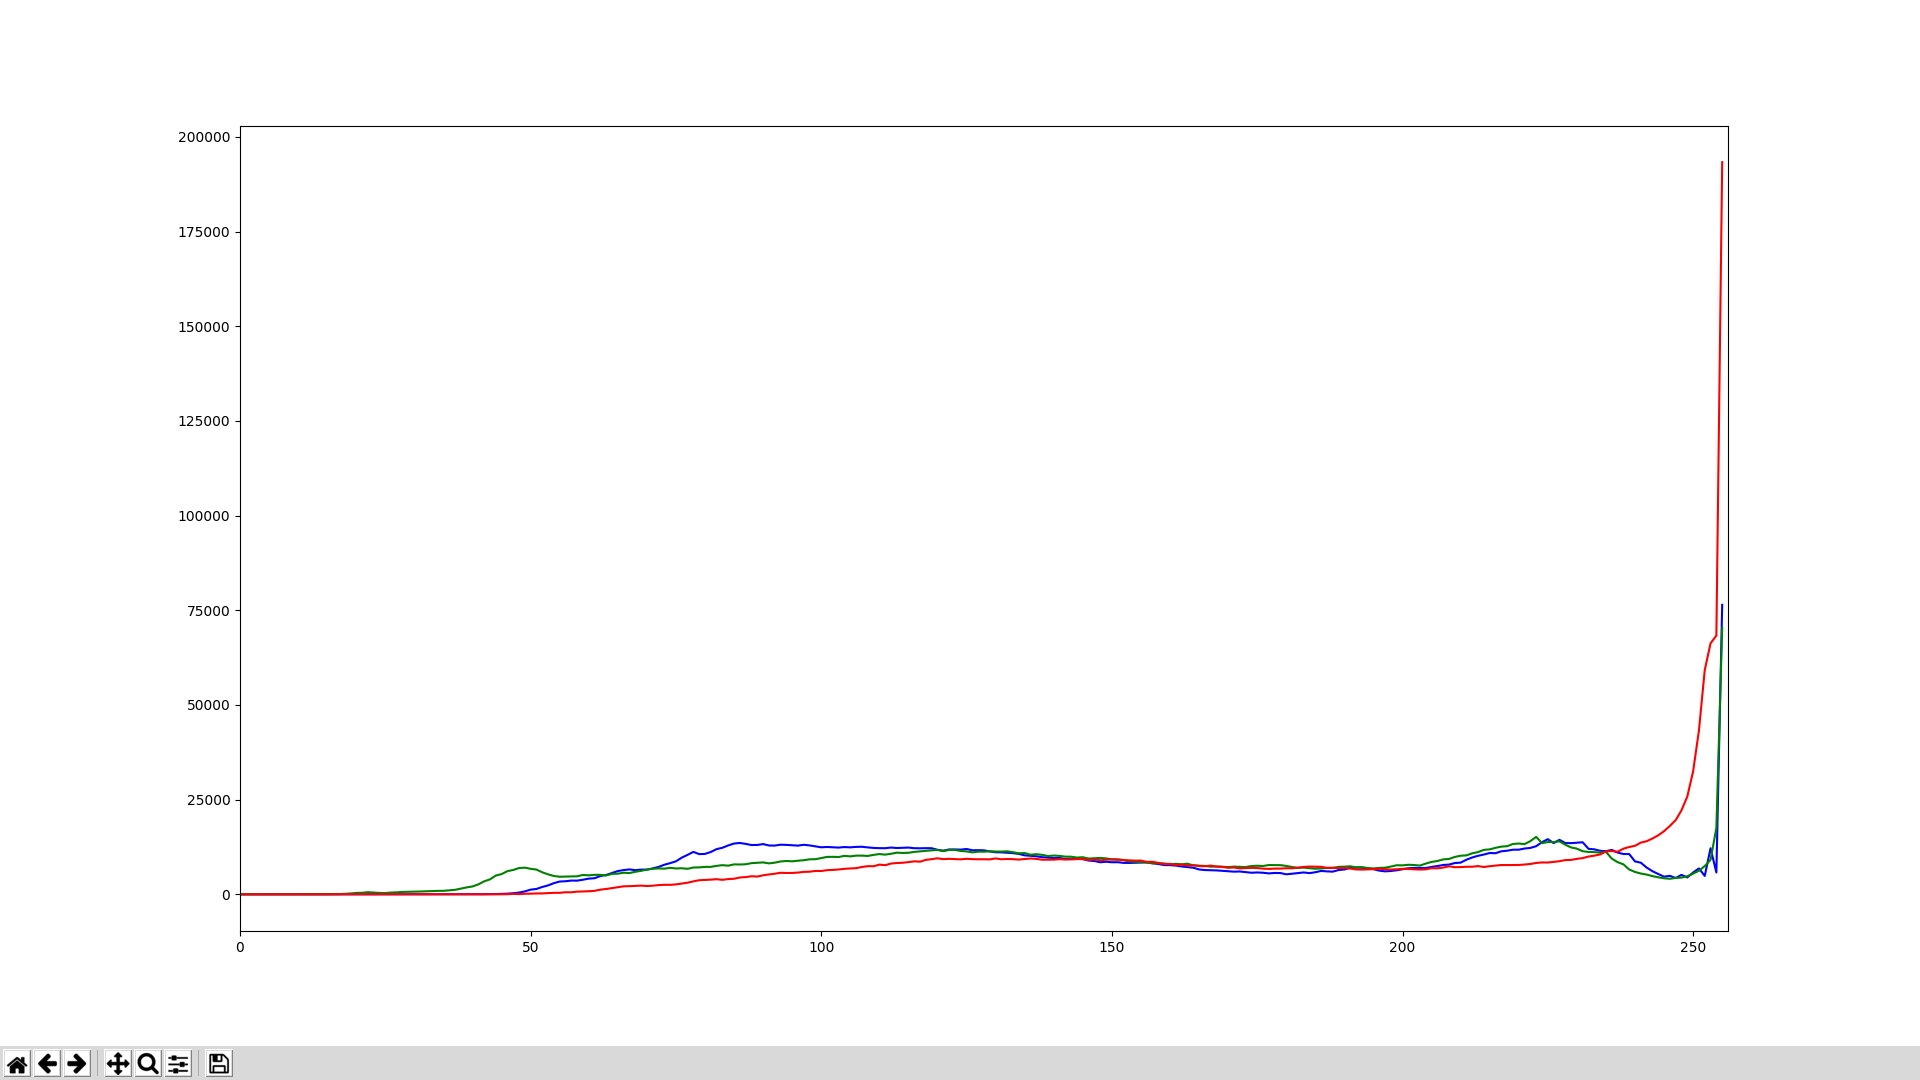
\includegraphics[width=0.75\textwidth]{2D-histrogram.png}
        \end{center}
        \newpage \noindent
        Wenn man für das selbe Bild nun ein 3D Histogramm generiert gewinnt man eine Dimension in der man eine weitere Information anzeigen
        kann. In diesem Beispiel bringt es die Information der genaue Verteilung von diesen drei Grundfarben in einem 3D Raum.
        \begin{center}
            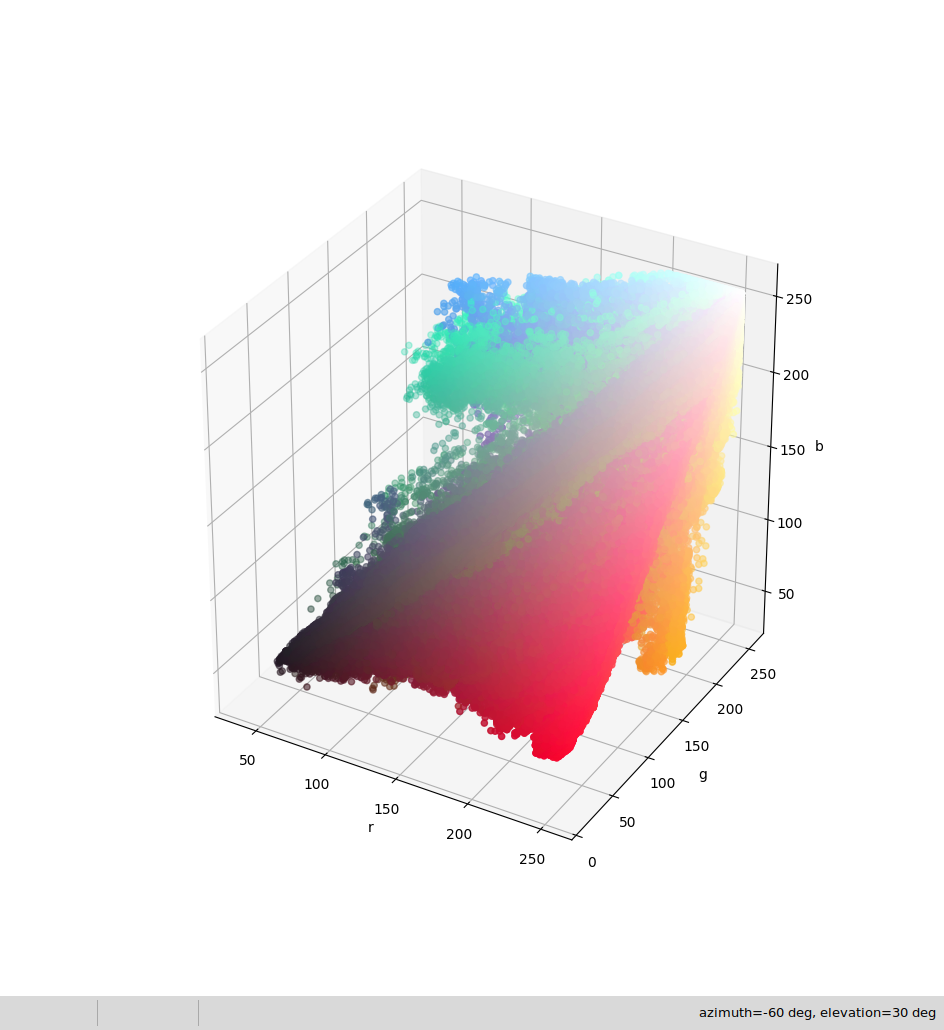
\includegraphics[width=0.75\textwidth]{3D-histogram.png}
        \end{center}
        \newpage \noindent
    \item{Karten:} \\ \\
        Karten werden seit Jahrtausenden verwendet um Distanzen und Landzüge zu visualisieren, jedoch kann man mit einer Karte wie John Snow
        im Jahre 1854 bewies, Ursachen für ausbrüche von Cholera ermitteln.\cite{bestvisualizations}
        \begin{center}
            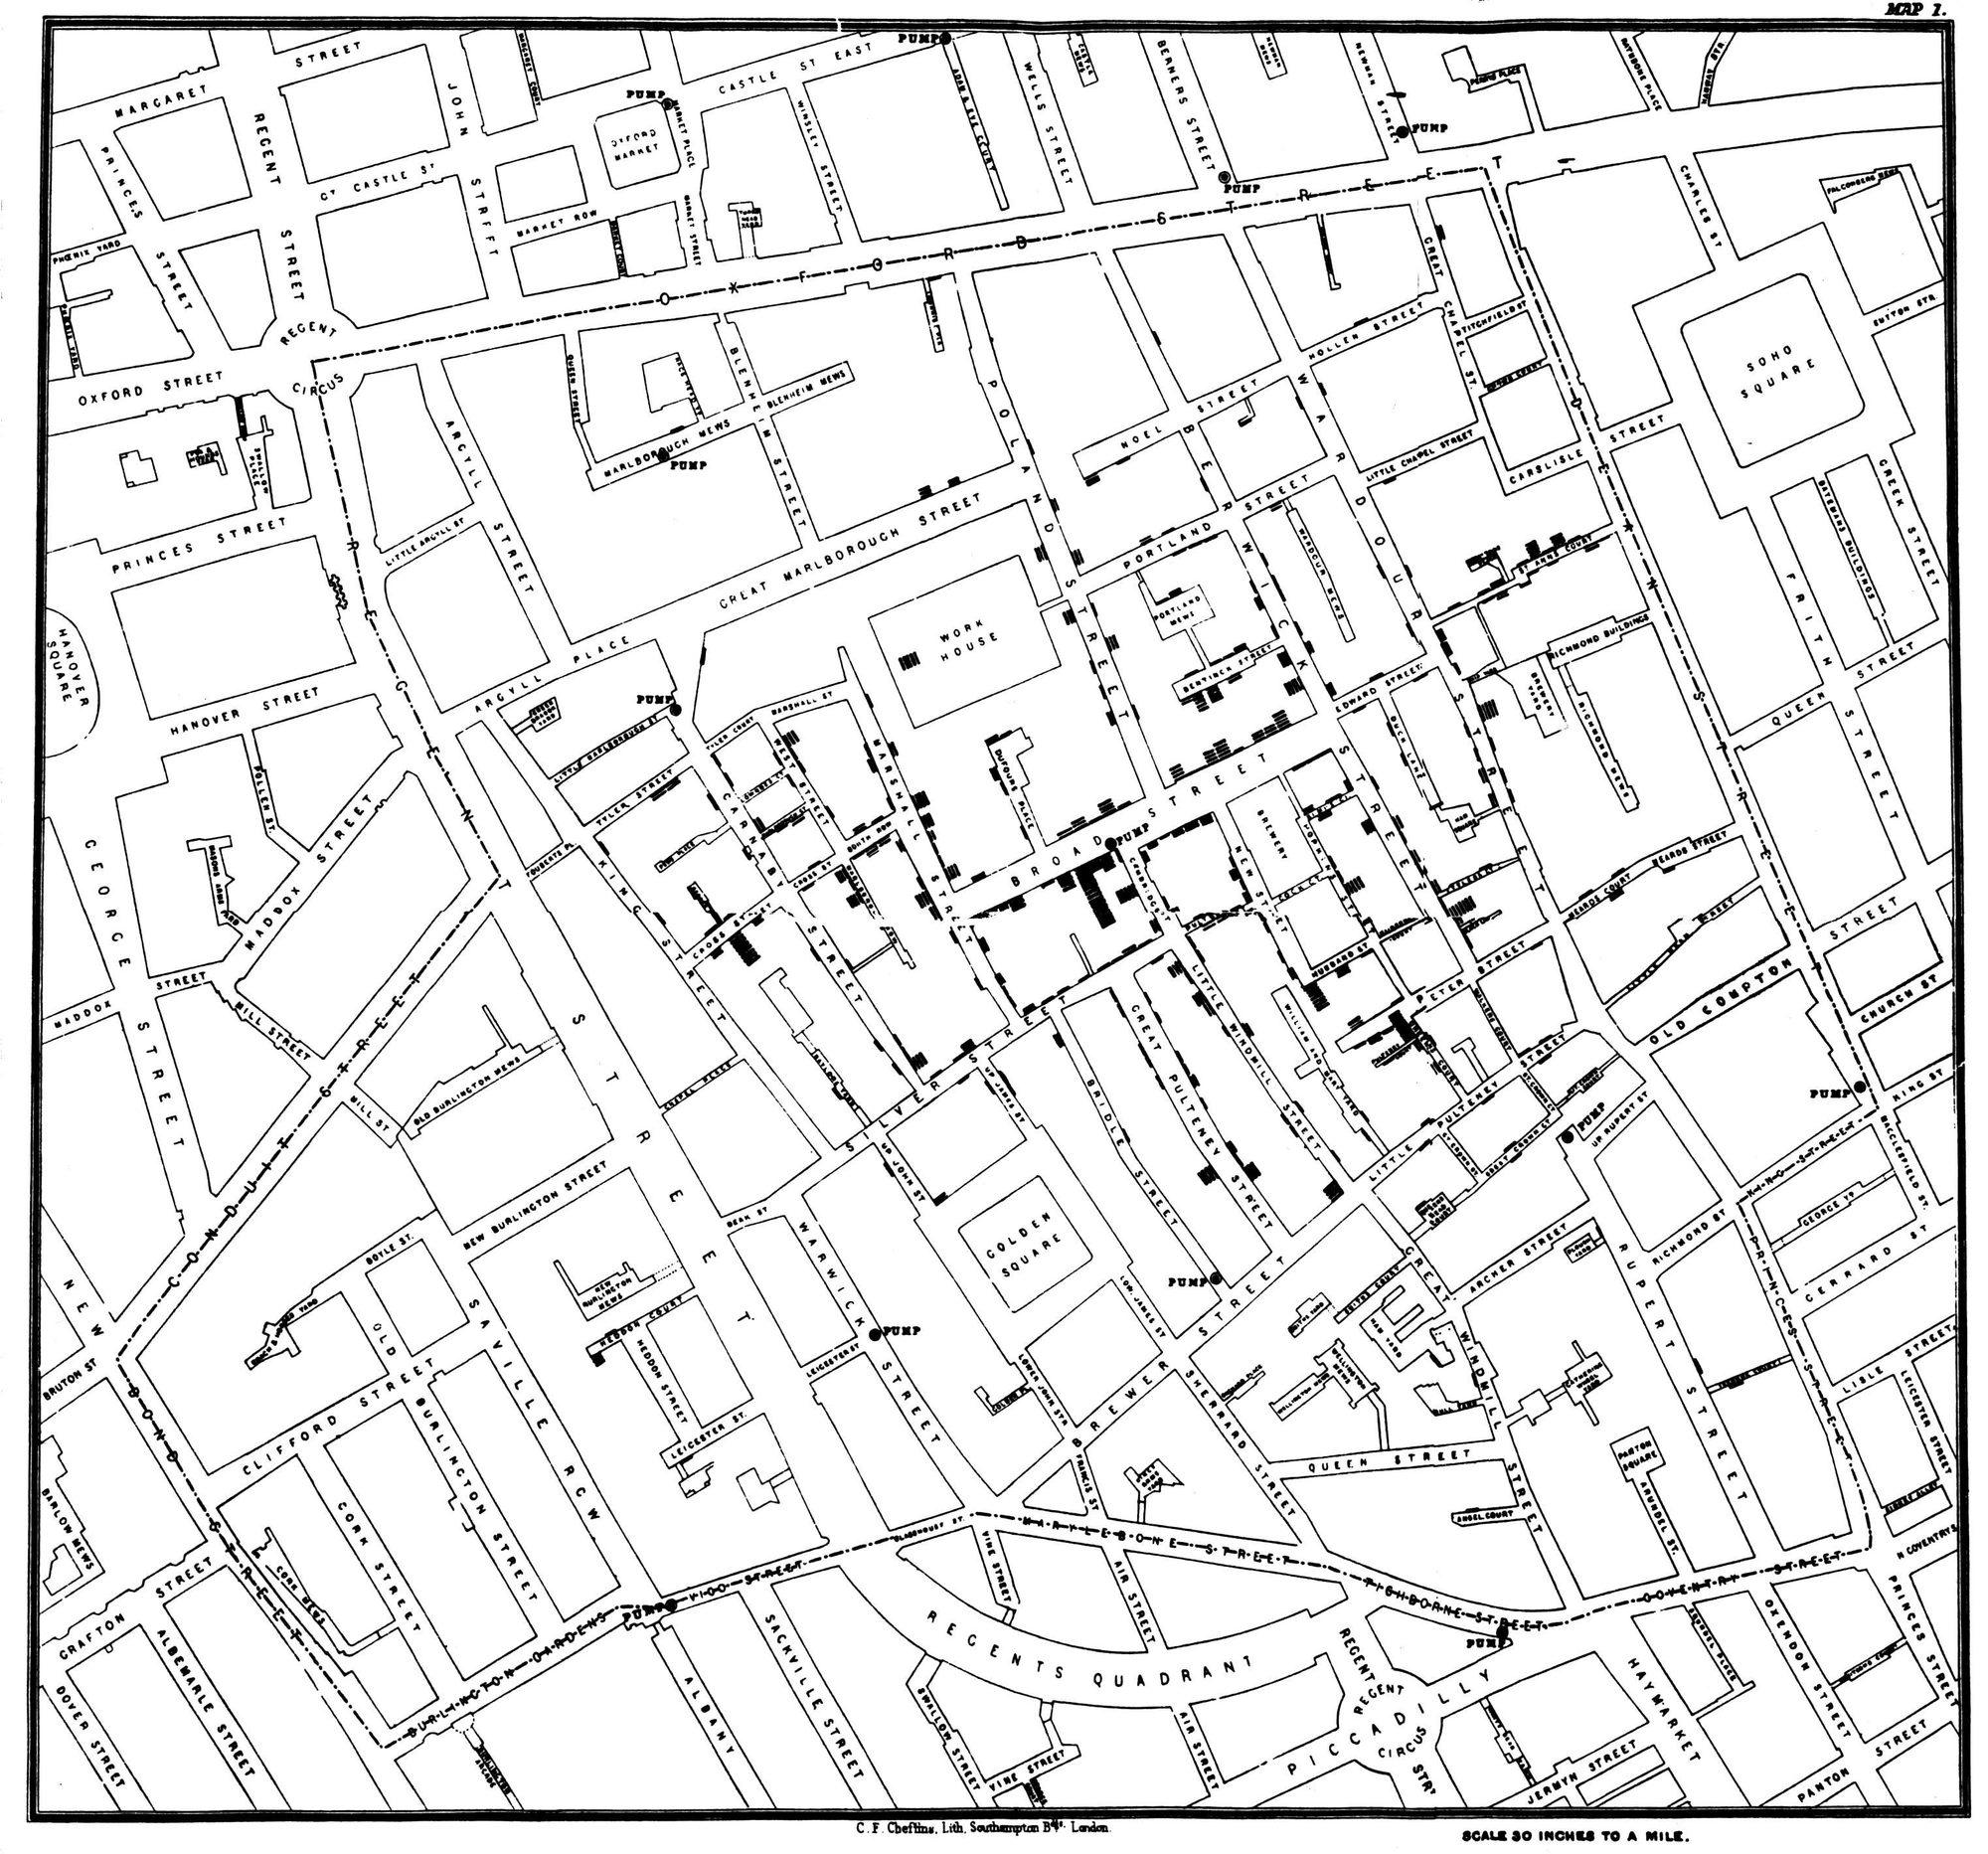
\includegraphics[width=0.75\textwidth]{2_snow-cholera-map.jpg}\cite{choleramap}
        \end{center}
        Auf dieser Karte wurden Regionen mit Balken versehen, welches die Häufigkeit des Ausbruchs von Cholera indizierten. Man
        konnte dadurch ermitteln das die Ursache der hohen ausbruchrate in den Distrikten die Wasserquelle war. Dieses wurde durch das
        Kanalsystem verpestet welches in die Quelle auslief.\cite{bestvisualizations}
        \newpage \noindent
    \item{Visualisierung im freien 2D-, 3D Raum:} \\ \\
        Die Visualisierung in einem freien 2D oder 3D Raum ohne vordefinierte Axen, ist relative neu und fokussiert sich auf das verarbeiten
        und visualisieren von Daten, die eventuell keine direkten Zusammenhänge haben. Der Bedarf für solche Visualisierungen entstand aus den
        Bereichen BigData und Machine Learning. Solche Daten müssen vor der Visualisierung erstmal Analysiert werden. Während der Analyse
        werden zusammenhänge in einer höheren oder niederen Ebene ermittelt. Meist müssen diese Informationen über andere Verfahren ermittelt
        werden, welche dann mit Algorithmen wie ''k-means'', ''octree'' oder anderen Methodiken in einem freien Raum visualisieren.
        \begin{center}
            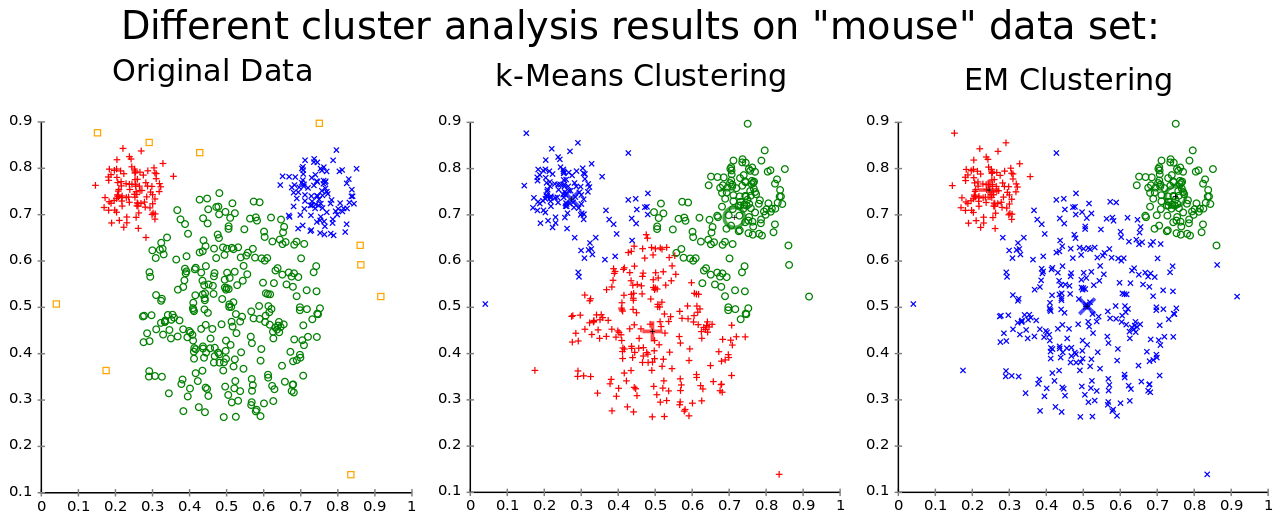
\includegraphics[width=0.75\textwidth]{ClusterAnalysis_Mouse.png}\cite{2dclustering}\\
            2D Clustering
            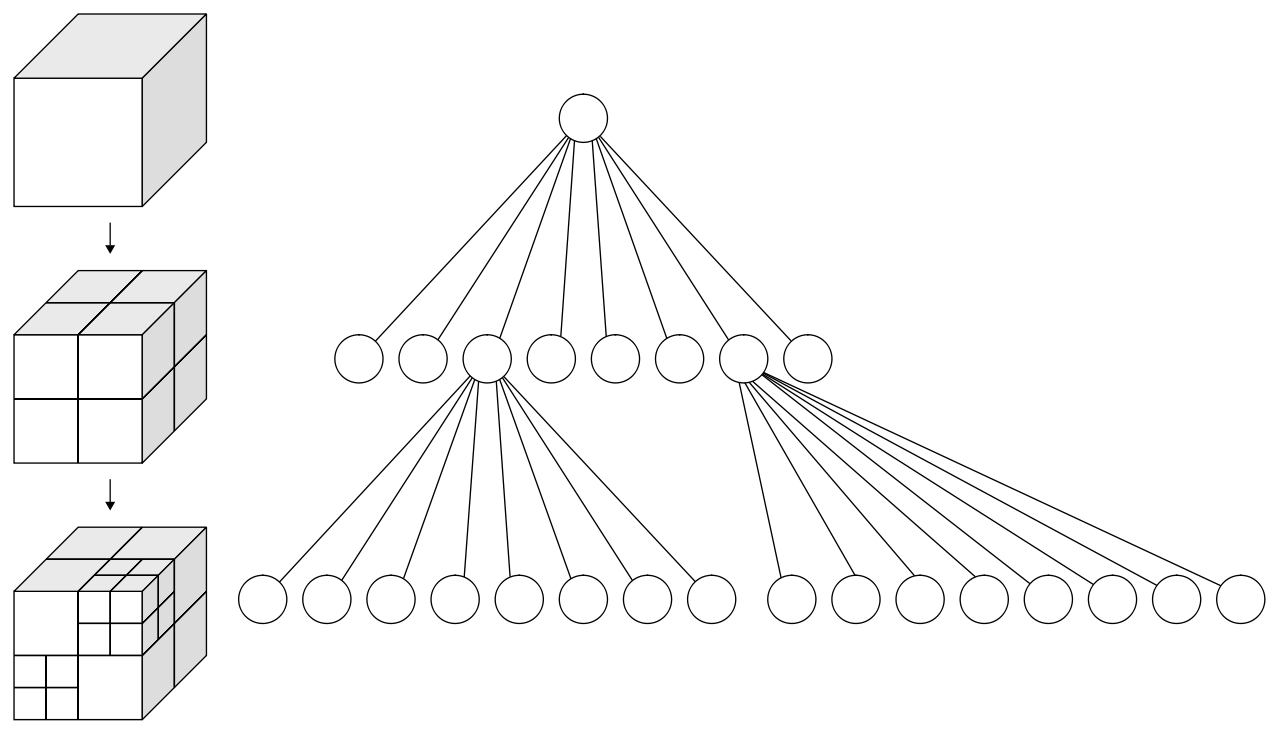
\includegraphics[width=0.75\textwidth]{1280px-Octree2.png}\cite{wikioctree}\\
            3D Octree
        \end{center}
\end{itemize}
\end{document}
